\documentclass{beamer}

\mode<presentation>{%
	\usetheme{Warsaw}
}

\usepackage[spanish]{babel}
\usepackage[utf8]{inputenc}
\usepackage[T1]{fontenc}
\usepackage{libertine}
\usepackage{beramono}
\usepackage{textcomp}
\usepackage{amsmath}
\usepackage{tabularx}
\usepackage{booktabs}
\usepackage{graphicx}

\setbeamertemplate{caption}[numbered]
\setbeamerfont{caption}{size=\footnotesize}

\newcolumntype{Y}{>{\centering\arraybackslash}X}

\title[Intuitive Theories of Mind: A Rational Approach to False Belief]{Intuitive Theories of Mind: \\ A Rational Approach to False Belief \\ \vspace{1ex} {\large Un Pequeño Análisis}}

\author[Grupo 10]{%
	Martín Fixman \and
	Axel Straminsky
}

\date{Primer Cuatrimestre 2016}

\begin{document}

\begin{frame}[fragile]
\titlepage{}
\end{frame}

\section{Introducción}

\begin{frame}[fragile]{Introducción}
Los niños pequeños suelen tener razonamientos falsos a ciertos problemas que parecen desconcentantes o dificiles de predecir para los adultos.

Esta presentación toma datos del paper de \textbf{Noah Goodman}\cite{goodman00} para demostrar que ambos modelos de razonamiento, tanto el de niños pequeños como el de niños mayores, pueden definirse como modelos Bayesianos de creencias falsas.
\end{frame}

\section{El Experimento}

\subsection{Pregunta}

\begin{frame}[fragile]{El Problema}
\begin{block}{\ Test de falsa creencia \vspace{1em}}
``Sally pone un juguete en una \textbf{canasta}, y luego va afuera a jugar. \\
Mientras ella juega, otra persona mueve el juguete a la \textbf{caja}. \\
Cuando Sally vuelve por su juguete, ¿dónde lo va a buscar?''
\end{block}

\vspace{1em}

\alt<2>{%
En este experimento, se le hace esta pregunta a niños de diferentes edades y se categorizan sus respuestas.

Como es esperado, los niños de hasta 3 ó 4 años de edad responden que Sally va a buscar el juguete en la caja, mientras que los mayores dicen que lo busca en la canasta.
}{}
\end{frame}

\begin{frame}
La habilidad de razonar acerca de los estados mentales de otras personas se conoce como \textbf{teoría de la mente}.

En particular, se estudia el fenómeno de las llamadas \textbf{creencias falsas}: la habilidad de inferir que otras personas tienen creencias que difieren de la realidad del mundo.
\end{frame}

\subsection{Diferencias en comportamiento}

\begin{frame}[fragile]
Dadas las respuestas a la pregunta, se puede pensar que hay sistemas de conceptos interrelacionados que generan predicciones y explicaciones en dominios particulares de experiencia\cite{murphy93}. Gracias a esto, podemos tomar dos perspectivas diferentes del mundo.

\vspace{2em}

\begin{columns}[T]
\begin{column}{.4\textwidth}
\alt<2->{%
	\textbf{\large Copy Theorist}

	Las creencias son siempre consistentes con el mundo.
}{}
\end{column}

\begin{column}{.5\textwidth}
\alt<3->{%
	\textbf{\large Perspective Theorist}

	Las creencias pueden ser cambiadas por perspectiva.

	Se pueden aceptar que se tienen creencias falsas.
}{}
\end{column}
\end{columns}

\end{frame}

\subsection{Racionalidad}

\begin{frame}[fragile]
Por investigaciones hechas anteriormente, se sabe que \textbf{el comportamiento humano es aproximadamente racional dentro de su contexto natural}\cite{anterson90}. Se puede sacar una de dos posibles conclusiones de este estudio:

\begin{itemize}
\item Una versión \textbf{fuerte}, donde los niños responden y aprenden a travez del desarrollo, y cada etapa de este se puede ver individualmente. Estos cambios son guiados por experiencia.
\item Una versión \textbf{débil}, donde solo el estado final de madurez es racional, y todos los estados anteriores se consideran irracionales.
\end{itemize}

\end{frame}

\begin{frame}

Empiricamente, los niños no adquieren de manera inmediata un entendimiento de lo que son las falsas creencias cuando son expuestos a evidencia incompatible con una posición CT\@.

La intuición sugiere que pasar a un modelo más complejo (Perspective Theorist), por la navaja de Occam, requiere evidencia más fuerte.
\end{frame}

\subsection{Interpretación Bayesiana}

\begin{frame}[fragile]{Una Interpretación Bayesiana}
Para formalizar esto, se especifican los dos modelos de creencias falsas, el del \textit{Copy Theorist} y el del \textit{Perspective Theorist}, que se pueden ver como \textbf{Redes Bayesianas}.

\begin{figure}
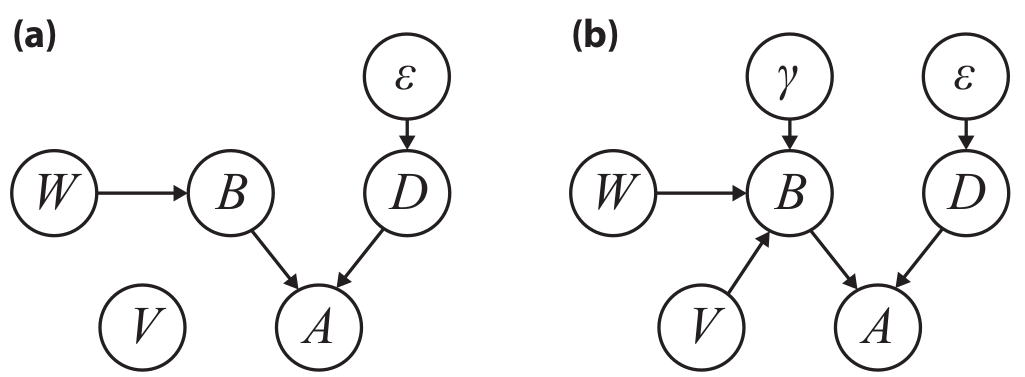
\includegraphics[width=0.6\textwidth]{imagenes/modelos.png}
\caption{Grafos de dependencia de nuestro modelo bayesiano. \textbf{(a)}: modelo CT \textbf{(b)} modelo PT.}
\end{figure}
\end{frame}

\begin{frame}
\vspace{1em}
Se usan tres variables observables.
\begin{description}
	\item[\texttt{\textbf{W}}] La posición final del juguete (\textbf{World}).  \\
		0 \textrightarrow{}  Posición original, 1 \textrightarrow{}  Posición nueva

	\item[\texttt{\textbf{V}}] Pudo ver Sally que el juguete fue movido? (\textbf{Access}). \\
		0 \textrightarrow{}  No, 1 \textrightarrow{}  Sí

	\item[\texttt{\textbf{A}}] A dónde va a buscar el juguete Sally (\textbf{Action}). \\
		0 \textrightarrow{}  Posición original, 1 \textrightarrow{}  Posición nueva
\end{description}

Y cuatro no observables (representan el estado mental)
\begin{description}
	\item[\texttt{\textbf{B}}] La ``creencia'' de Sally de la locación del juguete (\textbf{Belief}). \\
		0 \textrightarrow{} Posición original, 1 \textrightarrow{} Posición nueva

	\item[\texttt{\textbf{D}}] El deseo principal de Sally. (\textbf{Desire}) \\
		1 \textrightarrow{}  Encontrar el juguete, 0 \textrightarrow{}  Cualquier otra cosa

\end{description}
\end{frame}

\begin{frame}
\begin{description}
	\item[\(\boldsymbol{\varepsilon}\)] Probabilidad a priori de \texttt{\textbf{D}}.
	\item[\(\boldsymbol{\gamma}\)] Probabilidad a priori de \texttt{\textbf{B}}. Representa todas las razones por las que Sally podría cambiar de opinión: por ej., alguien le dijo que movieron el juguete.
\end{description}

Asumimos que ambas tienen priors Beta asimétricos.
\end{frame}

\begin{frame}

Las probabilidades condicionales están dadas por las siguientes tablas.

\begin{center}
\begin{columns}
\begin{column}{.2\textwidth}
\scalebox{.75}{%
\begin{tabular}{|c|c|c|}
\hline
\(P(A = 1 | B, D)\) & \(B\) & \(D\) \\ \hline
\(0\) & \(0\) & \(1\) \\
\(1\) & \(1\) & \(1\) \\
\(0.5\) & \(0\) & \(0\) \\
\(0.5\) & \(1\) & \(0\) \\
\hline
\end{tabular}
}
\end{column}
\begin{column}{.2\textwidth}
\scalebox{.75}{%
\begin{tabular}{|c|c|}
\hline
\( P_{CT} \left( B = 1 \mid W \right) \) & \( W \) \\ \hline
\( 0 \) & \( 0 \) \\
\( 1 \) & \( 1 \) \\
\hline
\end{tabular}
}
\end{column}
\begin{column}{.35\textwidth}
\scalebox{.75}{%
\begin{tabular}{|c|c|c|}
\hline
\( P_{PT} \left( B = 1 \mid W, V \right) \) & \( W \) & \( V \) \\ \hline
\( 0 \) & \( 0 \) & \( 1 \) \\
\( 1 \) & \( 1 \) & \( 1 \) \\
\( \gamma \) & \( 0 \) & \( 0 \) \\
\( \gamma \) & \( 1 \) & \( 0 \) \\
\hline
\end{tabular}
}
\end{column}
\end{columns}
\end{center}

\alt<2>{%
La probabilidad condicional para la acción describe el caso de un agente racional: una persona actuará racionalmente, dadas sus creencias, para satisfacer sus deseos.
}{}

\end{frame}

\section{Predicción}

\subsection{Predicción}
\begin{frame}

Existen 2 situaciones de ejemplo:

\begin{figure}[h!]
  \centering
    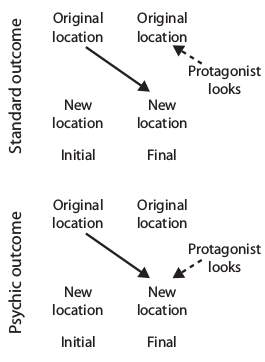
\includegraphics[width=0.4\textwidth]{imagenes/situaciones.jpg}
\end{figure}

En ambos casos W = 1 y V = 0 (el juguete está en la nueva ubicación, Sally no vio que movieron el juguete).

\end{frame}

\begin{frame}

Los modelos hacen predicciones opuestas:
%
%\begin{minipage}{0.1\textwidth}
%\begin{figure}
%  \raggedright
%    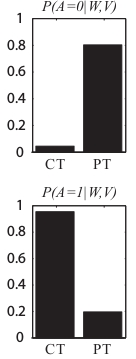
\includegraphics[width=2\textwidth]{imagenes/fig_b.jpg}
%\end{figure}
%\end{minipage}

%%TEXTO AL LADO
%\begin{minipage}[t]{\textwidth}
%  \begin{flushright}
%      El modelo CT
%
%  \end{flushright}
%\end{minipage}


\begin{minipage}{0.5\textwidth}
\begin{figure}[H]
	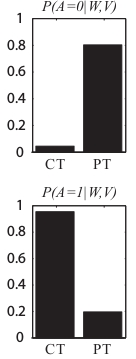
\includegraphics[width=0.5\textwidth]{imagenes/fig_b.jpg}
\end{figure}
\end{minipage} \hfill
\begin{minipage}{0.45\textwidth}
El modelo CT ``falla''   el test de falsa creencia prediciendo que Sally va a buscar el juguete en la \textbf{nueva} ubicación, mientras que el modelo PT ``pasa''   el test prediciendo la ubicación original.
\end{minipage}



\end{frame}

\begin{frame}
La racionalidad fuerte requiere que el agente haga un balance entre las teorías disponibles.

Se define el grado de creencia en cada modelo como su probabilidad a posteriori dada la experiencia previa:

\[
W_{PT/CT} = \log(P(PT|X)/P(CT|X))
\]

\end{frame}


\begin{frame}

\[
W_{PT/CT} = \log(P(PT|X)/P(CT|X))
\]

Cuando $W_{PT/CT}$ es muy negativo, el agente se comporta como si fuera un Copy Theorist puro. Si la evidencia se acumula y $W_{PT/CT}$ se vuelve muy positivo, el agente se comporta como un Perspective Theorist.


\end{frame}


\begin{frame}

\begin{figure}
	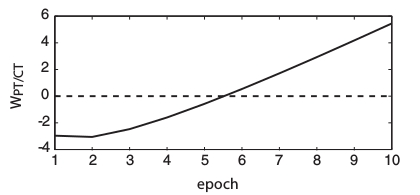
\includegraphics[width=0.6\textwidth]{imagenes/log_posterior.jpg}
\end{figure}

\end{frame}

\begin{frame}

\begin{figure}
	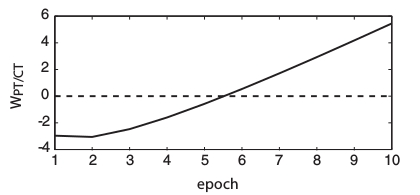
\includegraphics[width=0.6\textwidth]{imagenes/log_posterior.jpg}
\end{figure}

Cada época consiste en sucesiones de (W,V,A) observados, y codifican la asunción de que el acceso visual generalmente está disponible, y que, para las instancias en las que no está disponible, el protagonista generalmente tiene la creencia correcta.

\end{frame}



\end{document}
